
% !TEX encoding = UTF-8 Unicode

% Example of the Memoir class, an alternative to the default LaTeX classes such as article and book, with many added features built into the class itself.

\documentclass[10pt,a4paper,x11names]{memoir} % for a long document
%\documentclass[12pt,a4paper,article]{memoir} % for a short document
\usepackage{makeidx}
\usepackage{xparse,amsmath}
\usepackage{latexsym}
\usepackage{wasysym}
\usepackage{tabto}
\makeindex
\usepackage[utf8]{inputenc} % set input encoding to utf8
\usepackage{moreverb}
\usepackage{graphicx}
\usepackage{longtable}
\usepackage{ascii}
\usepackage{appendix}
\usepackage{smartdiagram}
\usesmartdiagramlibrary{additions}
\usetikzlibrary{shapes,arrows,chains,positioning}
\usepackage{xcolor}
\definecolor{orange}{rgb}{1,0.5,0}
\definecolor{salmon}{HTML}{AF3235}
\usepackage{listings}
\usepackage{wrapfig}

\usepackage{hyperref}
\hypersetup{
	bookmarks=true,         % show bookmarks bar?
	unicode=false,          % non-Latin characters in Acrobat’s bookmarks
	pdftoolbar=false,        % show Acrobat’s toolbar?
	pdfmenubar=true,        % show Acrobat’s menu?
	pdffitwindow=false,     % window fit to page when opened
	pdfstartview={FitH},    % fits the width of the page to the window
	pdftitle={Qlib documentation},    % title
	pdfauthor={Jacob Navia},     % author
	pdfsubject={Qlib documentation},   % subject of the document
	pdfcreator={Jacob Navia},   % creator of the document
	pdfproducer={TeXStudio + pdflatex}, % producer of the document
	pdfkeywords={CEPHES, C Language}, % list of keywords
	pdfnewwindow=true,      % links in new PDF window
	colorlinks=true,       % false: boxed links; true: colored links
	linkcolor=blue,          % color of internal links (change box color with linkbordercolor)
	citecolor=blue,        % color of links to bibliography
	filecolor=blue,         % color of file links
	urlcolor=blue        % color of external links
}
%\usepackage{MinionPro}
%\usepackage{multicolumn}
%\usepackage{tikz}
%\usepackage{utopia}
%\usepackage[explicit]{titlesec}
% Provide the command \fpeval as a copy of the code-level \fp_eval:n.
\usepackage{expl3}[2012-07-08]
\ExplSyntaxOn
\cs_new_eq:NN \fpeval \fp_eval:n
\ExplSyntaxOff
%\lstset{language=C,basicstyle=\ttfamily,numbers=left,numberstyle=\tiny,commentstyle=\white}
% Don't forget to read the Memoir manual: memman.pdf

%%% Examples of Memoir customization
%%% enable, disable or adjust these as desiredƒ

%%% PAGE DIMENSIONS
% Set up the paper to be as close as possible to both A4 & letter:
%\settrimmedsize{297mm}{210mm}{*} % letter = 11in tall; a4 = 210mm wide
%\setlength{\trimtop}{0pt}
%\setlength{\trimedge}{\stockwidth}
%\addtolength{\trimedge}{-\paperwidth}
%\settypeblocksize{*}{\lxvchars}{1.618} % we want to the text block to have golden proportionals
%\setulmargins{50pt}{*}{*} % 50pt upper margins
%\setlrmargins{*}{*}{1.618} % golden ratio again for left/right margins
%\setheaderspaces{*}{*}{1.618}
%\setheadfoot{\onelineskip}{2\onelineskip}
%\checkandfixthelayout
% ------------------------------------------------------------------lstlisting setup
\lstset{language=C,commentstyle=\color{violet}\itshape\small}
\lstset{numbers=left, numberstyle=\tiny,numbersep=5pt}
\lstset{fontadjust=true}
%\lstset{basicstyle=\ttfamily\small}
\lstset{breaklines=true}
\lstset{tabsize=4}
\lstset{showstringspaces=false}
\lstset{columns=flexible}
%\lstset{literate={<=}{{$\leq$}}1 {>=}{{$\geq$}}1 {!=}{{$\neq$}}1}
%\lstset{firstnumber=last}
\lstset{literate=[*]{>=}{{$\geq$}\ }3 {<=}{{$\leq$\ }}2{[}{[}1 {!=}{{$\neq$\ }}2 {->}{{$\rightarrow$}}2}
\lstset{moredelim=[is][\bfseries]{[*}{*]}}
\lstset{basicstyle=\ttfamily\small}
\lstset{ escapeinside={ {(@}{@)} } }

\settrimmedsize{297mm}{210mm}{*}
\setlength{\trimtop}{0pt}
\setlength{\trimedge}{\stockwidth}
\addtolength{\trimedge}{-\paperwidth}
\settypeblocksize{634pt}{400pt}{*}
\setulmargins{4cm}{*}{*}
\setlrmargins{40mm}{*}{*}
\setmarginnotes{17pt}{51pt}{\onelineskip}
\setheadfoot{\onelineskip}{2\onelineskip}
\setheaderspaces{*}{2\onelineskip}{*}
\checkandfixthelayout
% This is from memman.pdf
%%% \maketitle CUSTOMISATION
% For more than trivial changes, you may as well do it yourself in a titlepage environment
\pretitle{\begin{center}\sffamily\huge}
	\posttitle{\par\end{center}\vskip 0.5em}

%%% ToC (table of contents) APPEARANCE
\maxtocdepth{subsection} % include subsections
\renewcommand{\cftchapterpagefont}{}
\renewcommand{\cftchapterfont}{}     % no bold!

%%% HEADERS & FOOTERS
\pagestyle{ruled} % try also: empty , plain , headings , ruled , Ruled , companion

%%% CHAPTERS
\chapterstyle{hangnum} % try also: default , section , hangnum , companion , article, demo

\renewcommand{\chaptitlefont}{\Huge\sffamily\raggedright} % set sans serif chapter title font
\renewcommand{\chapnumfont}{\Huge\sffamily\raggedright} % set sans serif chapter number font

%%% SECTIONS
\hangsecnum % hang the section numbers into the margin to match \chapterstyle{hangnum}
\maxsecnumdepth{subsection} % number subsections

\setsecheadstyle{\Large\sffamily\raggedright} % set sans serif section font
\setsubsecheadstyle{\large\sffamily\raggedright} % set sans serif subsection font

%% END Memoir customization
\newcommand{\raisedrule}[2][0em]{\leaders\hbox{\rule[#1]{1pt}{#2}}\hfill}
\newcommand{\Section}[1]{\section{#1}\label{#1}\addcontentsline{toc}}

\usepackage[T1]{fontenc}
%\usepackage[urw-garamond]{mathdesign}
\newcommand{\indexAC}[1]{\index{\texttt{#1}}}
\newcounter{entry}
\counterwithin{entry}{chapter}
\newcommand{\TOC}[1] {\addcontentsline{toc}{section}{\theentry\ \  #1} \textbf{\theentry\ \  #1} \par\stepcounter{entry}}

%\usepackage{duerer}
%\usepackage{tgchorus}
%\usepackage{arev}

\title{ \textsl{Qlib, technical documentation}}
\author{ \textsl{jacob navia}}
%\date{} % Delete this line to display the current date
\usepackage{xargs}
\usepackage{color}
%\renewcommandx*{\hrulefill}[2][0pt]{\leavevmode \leaders \hbox to 1pt{\rule[#1]{1pt}{#2}} \hfill \kern 0pt}
%\renewcommand*\familydefault{\sfdefault} %% Only if the base font of the document is to be sans serif

\renewcommandx*{\hrulefill}[2][1=0.3mm,2=0pt]{\leavevmode \leaders \hbox to 1pt{\rule[#2]{1pt}{#1}} \hfill \kern 0pt}
\definecolor{purple}{rgb}{0.42,0.12,1.0}
\newcommand{\EOF}{
	{\footnotesize EOF}
}
%_______________________________________________________________
\newcommand{\Null}{
	{\footnotesize NULL}
}
%
% this makes list spacing much better.
%
\newenvironment{ShorterItemize}{
	\begin{itemize}
		\setlength{\itemsep}{1pt}
		\setlength{\parskip}{0pt}
		\setlength{\parsep}{0pt}}{\end{itemize}
}
%______________________________________________
\newcommand*{\titleJT}{\begingroup% Jan Tschichold: typographer
	%\FSfont{5gm} % FontSite Garamond
	\drop = 0.08\textheight \vspace*{\drop}
	\hspace*{0.3\textwidth} {}\\[1\drop]
	\hspace*{0.2\textwidth}
	{\HUGE\itshape\raggedleft Qlib: Technical documentation}\par \vspace{13cm} {\raggedleft\Huge\itshape jacob navia\par} \vfill \hspace*{0.3\textwidth}{\Large \raggedleft }\\[0.5\baselineskip] \hspace*{0.3\textwidth}{\Large } \vspace*{\drop} \endgroup}
\newlength{\drop}
%_
\usetikzlibrary{arrows}
\usepackage[T1]{fontenc}
\usepackage{tgpagella}
\usepackage{dtk-logos}


\begin{document}
\lstset{moredelim=[is][\bfseries]{[*}{*]}}
\setcounter{tocdepth}{5}
\setcounter{entry}{1}
\pagestyle{empty} \titleJT
\cleardoublepage
\pagestyle{headings}
\tableofcontents

\definecolor{mGreen}{rgb}{0,0.6,0}
\definecolor{mGray}{rgb}{0.5,0.5,0.5}
\definecolor{mPurple}{rgb}{0.58,0,0.82}
\definecolor{backgroundColour}{rgb}{0.95,0.95,0.92}

\lstdefinestyle{CStyle}{
	backgroundcolor=\color{backgroundColour},
	commentstyle=\color{mGreen},
	keywordstyle=\color{magenta},
	numberstyle=\tiny\color{mGray},
	stringstyle=\color{mPurple},
	basicstyle=\footnotesize,
	breakatwhitespace=false,
	breaklines=true,
	captionpos=b,
	keepspaces=true,
	numbers=left,
	numbersep=5pt,
	showspaces=false,
	showstringspaces=false,
	showtabs=false,
	tabsize=2,
	language=C
}
\lstset{language=C,numbers=left}
\chapter{Foreword}
This is a public release of my version of the CEPHES Mathematical Library. This work is based on the work of Stephen L Moshier, the author of the CEPHES Mathematical Library.

The copyright notice of that library is as follows:
\begin{verbatim}
   Some software in this archive may be from the book _Methods and
Programs for Mathematical Functions_ (Prentice-Hall or Simon & Schuster
International, 1989) or from the Cephes Mathematical Library, a
commercial product. In either event, it is copyrighted by the author.
What you see here may be used freely but it comes with no support or
guarantee.

The two known misprints in the book are repaired here in the
source listings for the gamma function and the incomplete beta
integral.


Stephen L. Moshier
moshier@na-net.ornl.gov
\end{verbatim}

Since the author allowed me to use his work freely, I have written a new version of it. The main differences from the original code are:
\begin{itemize}
	\item It is a 64 bit library. The last version that I know of it, was a 32 bit library with 144 bits. This version is a 64 bit one, using 448 bits.
	\item The four operations have been rewritten in pure assembler, making this version very fast. There are two versions of them: One in 64 bit x86-64 assembler, and the other in 64 bit ARM-64 assembler, what allows it to run in the raspberry pi and the 
	Apple Macintosh (with Apple's CPUs).
	\item The precision has been improved in many functions, and a new set of constants have been added with 448 bit precision.
	\item The documentation has been rewritten in the LATEX
	 system.
\end{itemize}

This software is very old. I have found a comment in studt.c like this:
\begin{verbatim}
/*  STUDNT.C    24 NOV 83

C       STUDNT.FOR      LATEST REV: 31 AUG 77
C               SLM, 31 AUG 77
C
C   EVALUTATES INTEGRAL OF STUDENT'S T DISTRIBUTION FROM
C   MINUS INFINITY TO T
C
C       USAGE:
C   CALL STUDNT(K,T,P)
C
C   K = INTEGER NUMBER OF DEGREES OF FREEDOM
C   T = RANDOM VARIABLE ARGUMENT
C   P = OUTPUT AREA
C
C   THE DENSITY FUNCTION IS
C   A*Z**-(K+2)/2,
C   WHERE Z = 1 + (T**2)/K
C   AND A = GAMMA((K+1)/2)/(GAMMA(K/2) * SQRT(K*PI)).
C   THE INTEGRAL IS EVALUATED IN CLOSED FORM BY INTEGRATION BY
C   PARTS.  THE RESULT IS EXACT, TO WITHIN ROUNDOFF ERROR.
C
C   SUBROUTINE LGAM, LOG OF GAMMA FUNCTION, IS NEEDED.
*/

\end{verbatim}
Mr Moshier has been working in this library since 1977. And it is a testament to the longevity of the 
software written in the C language that more than 40 years later it continues to run like new. C is not "the new language of the day", it
is a tried and tested language where you can build software that will run for decades.

Almost all of these functions were written by Stephen L. Moshier. These files have a copyright notice that begins in 1984 or 1985.
\begin{verbatim}
	* Cephes Math Library Release 2.3:  March, 1995
	* Copyright 1985, 1995 by Stephen L. Moshier
	
\end{verbatim}
I have revised the algorithms of some functions, added some (catalan, AGM, for instance) reformatted the code, but essentially this work is based on SLM's work.
\begin{verbatim}
/*
* Revision history:
*
* SLM,  5 Jan 84   PDP-11 assembly language version
* SLM,  2 Mar 86   fixed bug in asctoq()
* SLM,  6 Dec 86   C language version
* JN    1995-2011  Many improvements, modifications, etc
* JN    2017       Ported to ARM64
* JN    2021       Ported to Apple's M1
*/
\end{verbatim}
I have tested this version in three machines:
\begin{enumerate}
\item A PC with windows (16GB RAM, AMD Ryzen Windows 10) 
\item  A Macintosh (mac-mini Apple M1, 16GB RAM, Mac OS X)
\item  A Raspberry pi (8GB RAM and ARM64 CPU, Linux)
\end{enumerate}

\chapter{Data types}
This library features 8 bytes numbers, with a mantissa of seven 64 bits numbers and a header of 64 bits where the sign and the exponent are stored. This is a design for maximal speed, where space considerations are mostly ignored. The four operations are written entirely in ARM64/x86\_64 assembler. This allows to increase speed by a factor of 30 relative to a high level language like C. Built upon this assembler core functionality the module uses an adapted version of the CEPHES mathematical library written by Stephen L. Moshier. All higher order functions like logarithm, square root , exponential function etc, are written in C using the core functions.
\section{Data types}
Numbers are represented using the following structure:
\begin{lstlisting}
	typedef struct tagQfloat {
		int sign;                                      // 32 bits sign...
		unsigned int exponent;                         // 32 bits exponent
		unsigned long long mantissa[MANTISSA_LENGTH];  // 7 * 64 = 448 bits mantissa
	} Qfloat;
\end{lstlisting}

This differs completely of Mr Moshier representation as an undifferentiated table of integers. Access to exponent
and sign is clearer. All the library has been rewritten to use this structure. 

One problem in this transformation was that since numbers were a table of integers, they were always passed by reference, since tables are always passed as a reference to the first member in C. To keep this and avoid inefficiencies when passing numbers by value, all local variables and numbers are declared as tables of one element: instead of \verb,Qfloat x;, all the functions in the library use \verb,Qfloat x[1];, what is actually exactly the same, but since the second declaration will be understood as a table, it will be passed by reference in all calls.

All constants were recalculated for 64 bits and correctly rounded, and the precision in several functions was extended.
\section{Implementations}
Two assembler implementations exist: one for the x86\_64 and another for the ARM64 architectures. They are implemented essentially in the \verb,qasm-xxx, modules. There 3 of them: the \verb,aarch64, module for linux with ARM64, \verb,arm64, for Apple under ARM64, and x86\_64 for linux  under x86.
\section{Software organization}
Each function is implemented in  his own file. For instance qsqrt.c implements the square root, etc. 
There are several sub-directories:
\begin{itemize}
	\item \texttt{doc} Documentation in Latex
	\item \texttt{aarch64} Assembly programs for the linux aarch64 architecture (raspberry pi, rock64).
	\item \texttt{arm64} Apple's M1 series assembly programs.
	\item \texttt{x86-64} PC assembly programs
	\item \texttt{statslib} Statistics library in double precision
\end{itemize}


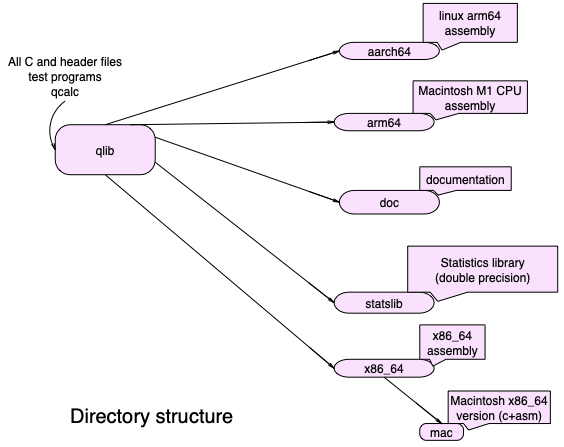
\includegraphics[scale=0.75]{directories.png}


\chapter{The functions}
\begin{longtable}{|p{1.5cm}|p{11.5cm}|}
	\caption{Qlib documentation}\\\hline
	\textbf{File}&\textbf{Function description}\\\hline\hline
	\endhead
	
	agm.c&This file implements the arithmetic geometric mean, written by 
	\verb,Tom Van Baak (tvb) www.LeapSecond.com/tools, and used to test the implementation in qfloat precision.\\\hline
	cmplx.c& This is the complex arithmetic module in double precision, used to calculate starting approximations for some functions.\\\hline
	qacosh.c& \TOC{Inverse hyperbolic cosine (qacosh)}
	
	{\footnotesize SYNOPSIS:}\vspace{-0.25cm}\index{qacosh}
	\begin{lstlisting}[numbers=none]
		int qacosh(x, y);
		qfloat *x; // input
		qfloat *y; // output
	\end{lstlisting}\vspace{-0.2cm}
	\par
	%\verb?acosh(x)  =  log( x + sqrt( (x-1)(x+1) )? 
	$$acosh(x) = log \left(x + \sqrt{(x-1)\times (x+1)}\right)$$
	\\\hline
	qagm.c & \TOC{Arithmetic Geometric Mean of two numbers (qagm)}
	
	{\footnotesize SYNOPSIS:}\vspace{-0.2cm}\index{qagm}
	\begin{lstlisting}[numbers=none]
		void qagm(x, y, r);
		qfloat *a; // input
		qfloat *g; // input
		qfloat *r; // output
	\end{lstlisting}\vspace{-0.2cm}
	
	 $x$ and $y$ is:\par
	$x_0 = x$ , 
	$y_0 = y$ \par
	$x_{n+1} = \frac{1}{2}  (x_n + y_n)$\par
	$y_{n+1} = \sqrt{x_n - y_n}$
	\\\hline
	qairy.c & \TOC{Airy functions}
	
	{\footnotesize SYNOPSIS:}\vspace{-0.2cm}\index{qairy}
	\begin{lstlisting}[numbers=none]
		int qairy( x, ai, aip, bi, bip );
		qfloat *x; // input
		qfloat *ai, *aip; // output
		qfloat *bi, *bip; // output
	\end{lstlisting}\vspace{-0.2cm}
	
	Solution of the differential equation\par
	$y''(x) = xy$.
	
	The function returns the two independent solutions Ai, Bi
	and their first derivatives Ai'(x), Bi'(x).
	
	Evaluation is by power series summation for small x, by asymptotic expansion for large x.
	
	{\footnotesize ACCURACY:}\par
	The asymptotic expansion is truncated at less than full working precision (only 105 digits).
	\\\hline
	qasin.c&\TOC{Inverse sine (qasin)}
	{\footnotesize SYNOPSIS:}\vspace{-0.2cm}\index{qasin}
	\begin{lstlisting}[numbers=none]
		int qasin( x, y );   int qasin( x, y );
		qfloat *x; // input
		qfloat *y; // output
	\end{lstlisting}\vspace{-0.2cm}
	
	This file implements \verb?asin(x)? and \verb?acos(x)?.\par
	\verb,qasin,  returns radian angle between -pi/2 and +pi/2 whose sine is x.
	
	%\verb?asin(x) = arctan (x / sqrt(1 - x^2))?
	$$asin(x) = arctan \left(\frac{1}{\sqrt{1-x^2} }\right)$$
	
	If $|x| > 0.5$ it is transformed by the identity\par
	
	% \verb?asin(x) = pi/2 - 2 asin( sqrt( (1-x)/2 ) )?.
	$$asin(x) = \frac{\pi}{2} - 2\times asin \left(\sqrt{\frac{(1-x)}{2}}\right)$$
	
	\verb,qacos:,   $$acos(x) = \frac{\pi}{2} - asin(x)$$
	\\\hline
	qasinh.c& \TOC{Inverse Hyperbolic sine (qasinh)}
	{\footnotesize SYNOPSIS:}\vspace{-0.2cm}\index{qasinh}
	\begin{lstlisting}[numbers=none]
		int qasinh( x, y );
		qfloat *x; // input
		qfloat *y; // output
	\end{lstlisting}\vspace{-0.2cm}
	$$asinh(x) = log\left(x+\sqrt{1+x^2}\right)$$
	For very large $x$,  $asinh(x)=log(x)+log(2)$
	\\\hline
	qatanh.c & \TOC{Inverse hyperbolic tangent (qatanh)}
	
	{\footnotesize SYNOPSIS:}\vspace{-0.2cm}\index{qatanh}
	\begin{lstlisting}[numbers=none]
		int qatanh( x, y );
		qfloat *x; // input
		qfloat *y; // output
	\end{lstlisting}\vspace{-0.2cm}
	Returns inverse hyperbolic tangent of argument.
	$$atanh(x) = 0.5 \times log \left( \frac{(1+x)}{(1-x)}\right)$$
	For very small x, the first few terms of the Taylor series
	are summed.
	\\\hline
	qatn.c& \TOC{Inverse circular tangent qatn}
	
	{\footnotesize SYNOPSIS:}\vspace{-0.2cm}\index{qatn}
	\begin{lstlisting}[numbers=none]
		int qatn( x, y );
		qfloat *x; // input
		qfloat *y; // output
	\end{lstlisting}\vspace{-0.2cm}
	Returns radian angle between $\frac{-\pi}{2}$and $\frac{+\pi}{2}$ whose tangent is x.
	
	Range reduction is from three intervals into the interval from zero to $\frac{\pi}{8}$.
	$$arctan(x)=\frac{x}{1 - \frac{x^2}{3 - \frac{4x^2}{5 - \frac{9x^2}{7-}}}} ... $$
	
	\\\hline
	qbeta.c &\TOC{Beta function (qbeta)}
	{\footnotesize SYNOPSIS:}\vspace{-0.2cm}\index{qbeta}
	\begin{lstlisting}[numbers=none]
		int qbeta( a, b, y );
		qfloat *a, *b; // inputs
		qfloat *y; // output
	\end{lstlisting}\vspace{-0.2cm}
	
	$$ beta(a,b) = \frac{\Gamma (a) \times \Gamma (b)}{\Gamma (a+b)}$$
	\\\hline
	qcalc.c& \index{qcalc }This is a calculator that features all functions of the package in an interactive way.\\\hline
	qcatalan.c& \TOC{Catalan (qcatalan)}
	{\footnotesize SYNOPSIS:}\vspace{-0.2cm}\index{qcatalan}
	\begin{lstlisting}[numbers=none]
		void qcatalan(n,result);
		qfloat *n; // input
		qfloat *result; // output
	\end{lstlisting}\vspace{-0.2cm}
	This returns the $n_{th}$ catalan number
	
	$$C_n=\frac{(2n)!}{(n+1)!\times n!}$$ These  numbers will be calculated using 128 bit integers up to $n=63$. For numbers above qfloat precision is used.
	\\\hline
	qcbrt.c& \TOC{Cubic root (qcbrt)}
	{\footnotesize SYNOPSIS:}\vspace{-0.2cm}\index{qcbrt}
	\begin{lstlisting}[numbers=none]
		int qcbrt( x, y );
		qfloat *x; // input
		qfloat *y; // output
	\end{lstlisting}\vspace{-0.2cm}
	This calculates the cubic root of a number that can be negative. A first approximation is calculated in double precision, then  the newton method is used for getting full precision.
	\\\hline 
	qconst.c& \TOC{Constants}
	
	A set of mathematical constants ($\pi$, $e$, $log(2)$, and several small numbers and fractions, all of them
	calculated to 132 digits precision.\index{qconst.c}\index{Constants}
	The constants were verified using the GP PARI calculator of Bordeaux's University. By a lucky coincidence the hexadecimal representation of floating point numbers is identical to qlib's. I have rounded all constant to 448 bits
	by using 140 decimal places in GP, what allowed me to see the next bits and round accordingly.
	
	qminusone \tabto{2.5cm}$-1$\tabto{4.2cm} qzero \tabto{6.2cm} $0$\tabto{7.4cm} qhalf  \tabto{9.7cm} $\frac{1}{2}$\par\vspace{0.2cm}
	qone \ \tabto{2.5cm}  $1$\tabto{4.2cm}   qtwo \tabto{6.2cm}  $2$\tabto{7.4cm} qthree \tabto{9.7cm}  $3$\par
	qfive \tabto{2.5cm} $5$\tabto{4.2cm}    qnine \tabto{6.2cm} $9$\tabto{7.4cm}  q32 \tabto{9.7cm} $32$\par\vspace{0.2cm}
	oneThird \tabto{2.5cm} $\frac{1}{3}$\tabto{4.2cm} qlog2 \tabto{6.2cm} $log(2)$\tabto{7.4cm}qinv\_log2 \tabto{9.7cm}$\frac{1}{log(2)}$\par\vspace{0.2cm}
	qsqrt2 \tabto{2.5cm}$\sqrt{2}$\tabto{4.2cm}qinv\_sqrt2\tabto{6.2cm}$\frac{1}{\sqrt{2}}$\tabto{7.4cm}
	oneopi\tabto{9.7cm}$\frac{1}{\pi}$\par \vspace{0.2cm}
	qpi\tabto{2.5cm}$\pi$\tabto{4.2cm} qPi\_Div\_2\tabto{6.2cm}$\frac{\pi}{2}$\tabto{7.4cm}
	qinv\_pi\tabto{9.7cm}$\frac{1}{\pi}$\par\vspace{0.2cm}
	qeul
	\footnote{This is the Euler-Mascheroni constant: 0,5772156649...}
	\tabto{2.5cm}$\gamma$\tabto{4.2cm}qlog10c\tabto{6.2cm}$log(10)$\tabto{7.4cm}qinv\_log10\tabto{9.7cm}$\frac{1}{log10}$\par\vspace{0.2cm}
	qmem1
	\footnote{This is used in Lambert's W function}
	\tabto{2.5cm}$-e^{-1}$\tabto{4.2cm}qexp\tabto{6.2cm}$e$\tabto{7.4cm}invSqrt2pi\tabto{9.7cm}$\frac{1}{\sqrt{\pi}}$\par
	qepsilon\tabto{2.5cm}$ 2^{-448}$
	\\\hline
	qcos.c& \index{qcos} \TOC{Cosinus (qcos)}
	
	{\footnotesize SYNOPSIS:}\vspace{-0.2cm}\index{qfcos}
	\begin{lstlisting}[numbers=none]
		int qfcos( x, y );
		qfloat *x; // input
		qfloat *y; // output
	\end{lstlisting}\vspace{-0.2cm}
	The cosinus is just $$\cos(x) = \sin \left(\frac{\pi}{2} - x\right)$$
	In this file the function $cos(x)-1$ (\verb,qcosm1,) is implemented using the Taylor series, useful for small $x$.
	\\\hline
	qcosh.c& 	\TOC{Hyperbolic cosine (qcosh)}\index{qcosh}
	
	{\footnotesize SYNOPSIS:}\vspace{-0.2cm}
	\begin{lstlisting}[numbers=none]
		int qcosh(x, y);
		qfloat *x; // input
		qfloat *y; // output
	\end{lstlisting}\vspace{-0.2cm}
	$$cosh(x)=\frac{exp(x)+exp(-x)}{2}$$
	\\\hline
	qei.c& 	\TOC{The exponential integral (qei)}
	
	{\footnotesize SYNOPSIS:}\vspace{-0.2cm}\index{qei}
	\begin{lstlisting}[numbers=none]
		qei( x, y );
		qfloat *x; // input
		qfloat *y; // output
	\end{lstlisting}\vspace{-0.2cm}
	$$Ei(x) = \int_{-\infty}^{x}\frac{e^t}{t} dt$$
	
	For values smaller than 32 this integral will be approximated by:
	$$Ei(x) = \delta + ln(x) + \sum_{n=1}^{\infty} \frac{x^n}{n \times n!}$$
	
	where $\delta$ is the  Euler–Mascheroni constant (0.577215664901...).
	
	For values > 32 SLM used the asymptotic expansion:
	$$x \times e^x \times Ei(x) = 1+\frac{2}{x^2}+\frac{6}{x^3} + ... \frac{n!}{x^n}$$
	\\\hline
	qellie.c&\TOC{Incomplete elliptic integral of the second kind (qellie)}
	
	{\footnotesize SYNOPSIS:}\vspace{-0.2cm}\index{qellie}
	\begin{lstlisting}[numbers=none]
		int qellie( phi, m, y );
		qfloat *phi, *m; // inputs
		qfloat *y;      // output
	\end{lstlisting}\vspace{-0.2cm}
	 Approximates the integral:
	$$ E(\phi,m) = \int_{0}^{\phi}\sqrt{1-m\times sin^2 \ t}\ dt $$
	
	of amplitude $\phi$ and modulus  $m$, using the arithmetic geometric mean algorithm.
	\\\hline
	qellik.c&\TOC{Incomplete elliptic integral of the first kind (qellik)}\index{qellik}
	{\footnotesize SYNOPSIS:}\vspace{-0.2cm}\index{ellik}
	\begin{lstlisting}[numbers=none]
		int qellik( phi, m, y );
		qfloat*phi, *m;   // inputs
		qfloat *y;        // output
	\end{lstlisting}\vspace{-0.2cm}
	
	 Approximates the integral:
	$$ F(\phi , m) = \int_{0}^{\phi} \frac{dt}{\sqrt{1-m\times sin^2 \ t}}$$
	\\\hline
	qellpe.c & \TOC{Complete elliptic integral of the second kind (qellpe)}
	{\footnotesize SYNOPSIS:}\vspace{-0.2cm}\index{qellpe}
	\begin{lstlisting}[numbers=none]
int qellpe(x, y);
qfloat *x; //input
qfloat *y; //output
	\end{lstlisting}\vspace{-0.2cm}
	Approximates the integral
	$$ E(m) = \int_{0}^{\frac{\pi}{2}} \sqrt{1 - m\ sin^2 t} \ dt$$
	\\\hline
	qellpj.c& \TOC{Jacobian Elliptic Functions (qellpi)}
	
	{\footnotesize SYNOPSIS:}\vspace{-0.2cm}\index{qellpi}
\begin{lstlisting}[numbers=none]
int qellpj( u, m, sn, cn, dn, ph );
qfloat *u, *m;             // inputs
qfloat *sn, *cn, *dn, *ph; // outputs
\end{lstlisting}\vspace{-0.2cm}
	
	
	Evaluates the Jacobian elliptic functions $sn(u|m)$, $cn(u|m)$,
	and $dn(u|m)$ of parameter $m$ between 0 and 1, and real
	argument $u$.
	
	These functions are periodic, with quarter-period on the
	real axis equal to the complete elliptic integral
	$ellpk(1.0-m)$.
	
	Relation to incomplete elliptic integral:
	If $u = ellik(\phi,m)$, then $sn(u|m) = \sin(\phi)$,
	and $cn(u|m) = \cos(\phi)$.  $\phi$ is called the amplitude of $u$.
	
	Computation is by means of the arithmetic-geometric mean
	algorithm, except when m is within 1e-9 of 0 or 1.  In the
	latter case with m close to 1, the approximation applies
	only for $\phi < \pi/2$.
	
	{\footnotesize{ACCURACY:}}  Truncated at 70 bits.
	\\\hline
	qellpk.c& \TOC{Complete elliptic integral of the first kind (qellpk)}
	
	{\footnotesize SYNOPSIS:}\vspace{-0.2cm}\index{qellpk}
	\begin{lstlisting}[numbers=none]
		int qellpk(x,y);
		qfloat *x; // input
		qfloat *y; //output
	\end{lstlisting}\vspace{-0.2cm}
	
	This approximates the integral:
	$$ K(m) = \int_{0}^{\frac{\pi}{2}}\frac{dt}{\sqrt{1-m\times sin^2\ t}}$$
	
	where $m = 1 - m1$, using the arithmetic-geometric mean method.
	
	The argument $m1$ is used rather than $m$ so that the logarithmic
	singularity at $m = 1$ will be shifted to the origin; this
	preserves maximum accuracy.
	
	$K(0) = \pi/2$.
	
	{\footnotesize ACCURACY:} Truncated at NBITS
	\\\hline
	qerf.c& \TOC{Error function (qerf)}
	
	{\footnotesize SYNOPSIS:}\vspace{-0.2cm}\index{qerf}
	\begin{lstlisting}[numbers=none]
		int qerf(x,y);
		qfloat *x; // input
		qfloat *y; // output
	\end{lstlisting}\vspace{-0.2cm}
	Calculates the error function.
	$$erf(x)=\frac{2}{\sqrt{\pi}} \ \int_{0}^{x} exp(-t^2)\ dt$$
	\\\hline
	qerfc.c&\TOC{Complementary error function}
	
	{\footnotesize SYNOPSIS:}\vspace{-0.2cm}\index{qerfc}
	\begin{lstlisting}[numbers=none]
		int qerfc(x,y);
		qfloat *x; // input
		qfloat *y; // output
	\end{lstlisting}\vspace{-0.2cm}
	This calculates:
	$$erfc(x)=\frac{2}{\sqrt{\pi}} \ \int_{x}^{\infty} exp(-t^2)\ dt = 1-erf(x)$$
	using two different continued fraction for arguments smaller than 4 and bigger than 4.
	\\\hline
	qexp.c& \TOC{The exponential function (qefexp)}
	
	{\footnotesize SYNOPSIS:}\vspace{-0.2cm}\index{qfexp}
	\begin{lstlisting}[numbers=none]
		int qfexp(x,y);
		qfloat *x; // input
		qfloat *y; // output
	\end{lstlisting}\vspace{-0.2cm}
	The exponential function ($e^z$)is implemented using the series $$e^z = \sum_{n=0}^{\infty} \frac{z^n}{n!}=1+\frac{z}{1}+\frac{z^2}{2!}+\frac{z^3}{3!} ...$$
	To achieve full precision this needs approx 30-40 iterations, depending on the argument. Arguments close to 1 need more iterations. This method is different from the one used by Mr Moshier: $$exp(x)=\frac{1+tanh(x)}{1-tanh(x)}$$
	The speed of the calculation was improved by 60\%. On the downside a loss of 1 ulps has been seen due to the long summation of the pre-calculated inverse factorials table.
	\\\hline
	qexp10.c& \TOC{Base 10 exponential function (qexp10)}
	
	{\footnotesize SYNOPSIS:}\vspace{-0.2cm}\index{qexp10}
	\begin{lstlisting}[numbers=none]
		int qexp10(x,y);
		qfloat *x; // input
		qfloat *y; // output
	\end{lstlisting}\vspace{-0.2cm}
	(Common antilogarithm).
	$$10^x=e^{x \times log(10)}$$
	\\\hline
	qexp2.c& \TOC{Base 2 exponential function (qexp2)}
	
	{\footnotesize SYNOPSIS:}\vspace{-0.2cm}\index{qexp2}
	\begin{lstlisting}[numbers=none]
		int qexp2(x,y);
		qfloat *x; // input
		qfloat *y; // output
	\end{lstlisting}\vspace{-0.2cm}
	Base 2 exponential function
	$$2^(x)=e^{x\times log(2)}$$
	\\\hline
	qexpm1.c& $e^x - 1$ \TOC{expm1 (qexpm1)}\index{qexpm1}
	{\footnotesize SYNOPSIS:}\vspace{-0.2cm}
	\begin{lstlisting}[numbers=none]
		int qexpm1(x,y);
		qfloat *x; // input
		qfloat *y; // output
	\end{lstlisting}\vspace{-0.2cm}
	Returns e (2.71828...) raised to the x power, minus 1.
	
	 If x is nearly zero, then the common expression exp(x) - 1.0 will suffer from catastrophic
	cancellation and the result will have little or no precision.  The \verb,expm1, function provides
	an alternative means to do this calculation without the risk of significant loss of precision.
	\\\hline
	qexpn.c& \TOC{Exponential integral (qexpn)}
	
	{\footnotesize SYNOPSIS:}\vspace{-0.2cm}
	\begin{lstlisting}[numbers=none]
		int qexpn(n,x,y);
		qfloat *n; // input
		qfloat *x; // input
		qfloat *y; // output
	\end{lstlisting}\vspace{-0.2cm}\index{qexpn}
	Evaluates the exponential integral:
	$$E_n(x)=\int_{1}^{\infty}\frac{e^{-xt}}{t^n}\ dt$$
	\\\hline
	qfac.c& \TOC{Factorial (qfact)}
	
	{\footnotesize SYNOPSIS:}\vspace{-0.2cm}
	\begin{lstlisting}[numbers=none]
		int qfact(x,y);
		qfloat *x; // input
		qfloat *y; // output
	\end{lstlisting}\vspace{-0.2cm}
	Calculates $n!$.
	\\\hline
	qfloor.c&\TOC{Floor (qfloor)}
	{\footnotesize SYNOPSIS:}\vspace{-0.2cm}
	\begin{lstlisting}[numbers=none]
		int qfloor(x,y);
		qfloat *x; // input
		qfloat *y; // output
	\end{lstlisting}\vspace{-0.2cm}
	
	Computes the largest integer not greater than x.
	\\\hline 
	qfltbi.c&\TOC{The qfltbi file}\index{qfltbi.c}
	This file contains all the low level routines that were rewritten in assembler. The main routines are:
	\begin{lstlisting}[numbers=none]
		addm( x, y )        add significand of x to that of y
		shdn1( x )          shift significand of x down 1 bit
		shdn8( x )          shift significand of x down 8 bits
		shdn16( x )         shift significand of x down 16 bits
		shup1( x )          shift significand of x up 1 bit
		shup8( x )          shift significand of x up 8 bits
		shup16( x )         shift significand of x up 16 bits
		divm( a, b )        divide significand of a into b
		mulm( a, b )        multiply significands, result in b
		mdnorm( x )         normalize and round off
	\end{lstlisting}
	\\\hline
	qflti.c&\TOC{Utilities}\index{qflti.c}
	qfloat precision utilities.
	\begin{lstlisting}[numbers=none]
		asctoq( string, q)  ascii string to q type
		etoq( d, q )        IEEE double precision to q type
		e24toq( d, q )      IEEE single precision to q type
		itoq( &l, q )       long integer to q type
		qabs(q)             absolute value
		qadd( a, b, c )     c = b + a
		qclear(q)           q = 0
		qcmp( a, b )        compare a to b
		qdiv( a, b, c )     c = b / a
		qifrac(x,&l,frac)   x to integer part l and q type fraction
		qfrexp( x, l, y )   find exponent l and fraction y between .5 and 1
		qldexp( x, l, y )   multiply x by 2^l
		qinfin( x )         set x to infinity, leaving its sign alone
		qmov( a, b )        b = a
		qmul( a, b, c )     c = b * a
		qmuli( a, b, c )    c = b * a, a has only 16 significant bits
		qisneg(q)           returns sign of q
		qneg(q)             q = -q
		qnrmlz(q)           adjust exponent and mantissa
		qsub( a, b, c )     c = b - a
		qtoasc( a, s, n )   q to ASCII string, n digits after decimal
		double qtoe(q,doround) convert q type to IEEE double precision
		qtoe24( q, &d )     convert q type to IEEE single precision
		qinv(src,result)    Inverse: result = 1/src. 
	\end{lstlisting}
	\\\hline
	\multicolumn{2}{c}{Conversions}\\\hline
	qflti.c& \TOC{Convert text to qfloat (asctoq)}\index{asctoq}
	
	{\footnotesize SYNOPSIS:}\vspace{-0.2cm}
	\begin{lstlisting}[numbers=none]
		int asctoq(const char *text, qfloat *output, char **pend);
	\end{lstlisting}
	
	The character string \verb,text, will be converted into qfloat, and the \verb,pend, pointer will point to the character right after the last digit. Scientific notation is supported.
	\\\hline
	qflti.c& \TOC{Convert qfloat to text (qtoasc)}\index{qtoasc}
	
	{\footnotesize SYNOPSIS:}\vspace{-0.2cm}
	\begin{lstlisting}[numbers=none]
int qtoasc(Qfloatp q,char *string,int width,int ndigs,int flags );
	\end{lstlisting}\vspace{-0.2cm} \par
	
	Formats the given number using the given width and number of digits after the decimal point. Numbers are rounded to the given
	precision.
	\\\hline
	qflti.c&\TOC{Conversion of double, float to qfloat (e2q e24toq)}
	
	{\footnotesize SYNOPSIS:}\vspace{-0.2cm}\index{etoq}\index{e24toq}
	\begin{lstlisting}[numbers=none]
		int etoq(double a,qfloat *b);
		int e24toq(float d,qfloat *b);
	\end{lstlisting}\vspace{-0.2cm} \par
	\verb,etoq, converts the double precision number $a$ into a qfloat. \verb,e24toq, converts a single
	precision one into a qfloat.
	\\\hline
	qflti.c& \TOC{Conversion of qfloat to double, float, and long double}
	
	{\footnotesize SYNOPSIS:}\vspace{-0.2cm}\index{qtoe}
	\begin{lstlisting}[numbers=none]
		double qtoe(Qfloatp x,int roundflag);
	\end{lstlisting}\vspace{-0.2cm} \par
	
	\verb,qtoe, converts the qfloat number $x$ into a double precision one. If \verb,roundflag, is not zero, rounding will be performed,
	otherwise the number is truncated.
	\\\hline
	qfltbi.c&\TOC{64 bit integer to qfloat}
	
	{\footnotesize SYNOPSIS:}\vspace{-0.2cm}\index{lltoq}
	\begin{lstlisting}[numbers=none]
		void lltoq(long long a,qfloat *b);
	\end{lstlisting}\vspace{-0.2cm} \par
	This function is written in assembler.
	\\\hline
	qflti.c& \TOC{Compare numbers}
	
	{\footnotesize SYNOPSIS:}\vspace{-0.2cm}\index{qcmp}
	\begin{lstlisting}[numbers=none]
		int qcmp(qfloat *a, qfloat*b);
	\end{lstlisting}\vspace{-0.2cm} \par
	Returns 1 if $a> b$, zero if $a = b$ or $-1$ if $a<b$.
	\\\hline
	qflti.c& \TOC{Integer part and fraction}
	
	{\footnotesize SYNOPSIS:}\vspace{-0.2cm}\index{qifrac}
	\begin{lstlisting}[numbers=none]
		void qifrac(Qfloatp x,long long *i,Qfloatp frac);
	\end{lstlisting}\vspace{-0.2cm} \par
	\verb,qifrac, will write into the location pointed by $i$ the integer part of $x$ and in $frac$ the fractional part. If the integer part doesn't fit into a 64 bit integer the result is \verb,0x7fffffffffffffff,.
	\\\hline
	\multicolumn{2}{c}{The four operations}
	\\\hline
	qflti.c& \TOC{Addition}\index{qadd}
	
	{\footnotesize SYNOPSIS:}\vspace{-0.2cm}
	\begin{lstlisting}[numbers=none]
		int qadd(qfloat *const a,qfloat *const b,qfloat *c);
	\end{lstlisting}\vspace{-0.2cm} $ c=b+a$.\par
	Returns 1 if the operation was done, zero if the exponent difference between the two numbers was beyond accuracy, $-1$ if an underflow occurred, and $-2$ if overflow was detected. In case of underflow the result (c) is zero, in case of overflow the result is the biggest possible number. In case the result would be beyond accuracy, the larger number is copied to the result.
	This procedure is written in assembly language.
	\\\hline
	
	qfltbi.c& \TOC{Subtraction}
	
	{\footnotesize SYNOPSIS:}\vspace{-0.2cm}\index{qsub}
	\begin{lstlisting}[numbers=none]
		int qsub(qfloat *const a,qfloat *const b,qfloat *c);
	\end{lstlisting}\vspace{-0.2cm}
	$ c=b-a$\par
	Returns the same integer codes as \verb,qadd,. This procedure is written in assembly language.
	\\\hline
	qflbi.c& \TOC{Multiplication}
	
	{\footnotesize SYNOPSIS:}\vspace{-0.2cm}\index{qmul}
	\begin{lstlisting}[numbers=none]
		void qmul(qfloat *const a,qfloat *const b,qfloat *c); 
	\end{lstlisting}\vspace{-0.2cm}
	$c=b\times a$.\par
	If an overflow occurs, it returns the biggest possible number in c. This procedure is written in assembly language.
	
	\\\hline
	qflbi.c& \TOC{Multiplication by a 64 bit integer}
	
	{\footnotesize SYNOPSIS:}\vspace{-0.2cm}\index{qmuli}
	\begin{lstlisting}[numbers=none]
		void qmuli(long long a,qfloat *const b,qfloat *c); 
	\end{lstlisting}\vspace{-0.2cm}
	$c=b\times a$.\par
	If an overflow occurs, it returns the biggest possible number in c. This procedure is written in assembly language.
	\\\hline
	qfltbi.c& \TOC{Division}
	
	{\footnotesize SYNOPSIS:}\vspace{-0.2cm}\index{qdiv}
	\begin{lstlisting}[numbers=none]
		int qdiv(qfloat *const a,qfloat *const b,qfloat *c);
	\end{lstlisting}\vspace{-0.2cm}
	$c=b/a$.\par
	This procedure is written in assembly language.
	\\\hline
	qfltbi.c&  \TOC{Assignment}
	
	{\footnotesize SYNOPSIS:}\vspace{-0.2cm}\index{qmov}
	\begin{lstlisting}[numbers=none]
		int qmov(qfloat *const a,qfloat *b);
	\end{lstlisting}\vspace{-0.2cm}
	$b=a$.\par
	This procedure is written in assembly language.
	\\\hline
	qflti.c&\TOC{Inverse}
	{\footnotesize SYNOPSIS:}\vspace{-0.2cm}\index{qmov}
	\begin{lstlisting}[numbers=none]
		int qinv(qfloat *const x,qfloat *y);
	\end{lstlisting}\vspace{-0.2cm}
	$$y=\frac{1}{x}$$
	\\\hline
	qfresf.c& \TOC{Fresnel integral}
	
	{\footnotesize SYNOPSIS:}\vspace{-0.2cm}\index{qfresnl}
	\begin{lstlisting}[numbers=none]
		int qfresnl( x, s, c );       int qfresng(x,f,g)
		qfloat *x; /* input */        qfloat *x; // input
		qfloat *s; /* output */       qfloat *f; // output
		qfloat *c; /* output */       qfloat *g; // output
	\end{lstlisting}\vspace{-0.2cm}
	Evaluates the Fresnel integrals:
	$$C(x)=\int_{0}^{x}cos\left(\pi/2 \times t^2\right)\ dt$$
	$$S(x)=\int_{0}^{x}sin\left(\pi/2 \times t^2\right)\ dt$$
	
	The integrals are evaluated by a power series for x < 1.
	For large x auxiliary functions $f(x)$ and $g(x)$ are employed
	such that:
	
	$$C(x) = 0.5 + f(x)\times sin\left( \frac{\pi}{2}\  x^2 \right) - g(x)\ cos\left( \frac{\pi}{2} \  x^2 \right)$$
	$$S(x) = 0.5 - f(x)\times cos\left( \frac{\pi}{2}\  x^2 \right) - g(x)\ sin\left( \frac{\pi}{2} \  x^2 \right)$$
	
	Routine \verb,qfresfg, computes f and g.
	
	{\footnotesize ACCURACY:}
	Series expansions are truncated at less than full working precision.
	\\\hline \TOC{ldexp and frexp}
	qfrexp.c&\index{qldexp}\index{qfrexp}
	{\footnotesize SYNOPSIS:}\vspace{-0.2cm}
	\begin{lstlisting}[numbers=none]
		void qldexp(x,n, y);               void qfrexp(x,n,y)
		qfloat *x; /* input  */            qfloat *x; // input
		long n;    /* input  */            int *n;    // output
		qfloat *y; /* output */            qfloat *y; // output
	\end{lstlisting}\vspace{-0.2cm}
	The \verb,qldexp, function multiplies $x$ by $2^n$ 
	The \verb,qfrexp, function breaks the input $x$ into a normalized fraction and an integral power of 2.
	\\\hline
	qgamma.c& \TOC{log of Gamma function}
	{\footnotesize SYNOPSIS:}\vspace{-0.2cm}\index{qlgam}
	\begin{lstlisting}[numbers=none]
		int qlgam(x,y);                    int qgamma(x,y)
		qfloat *x; /* input  */            qfloat *x; // input
		qfloat *y; /* output */            qfloat *y; // output
	\end{lstlisting}\vspace{-0.2cm}
	
	The function \verb,qlgam, calculates the natural logarithm of gamma function. The \verb,qgamma, function returns the value of the gamma function.
	\\\hline
	qhy2f1.c& \TOC{Hypergeometric $_2F_1$}
	{\footnotesize SYNOPSIS:}\vspace{-0.2cm}\index{qhy2f1}
	\begin{lstlisting}[numbers=none]
		int qhy2f1( a, b, c, x, y );
		qfloat *a,*b,*c,*x; // input
		qfloat *y; // output
	\end{lstlisting}\vspace{-0.2cm}
	$$hy_2f_1 = 1+\sum_{k=0}^{\infty}\frac{a(a+1)(a+2)\ ...(a+k)\ b(b+1)(b+2)\ ... (b+k)}{c(c+1)(c+2)\ ... (c+k)\times (k+1)!}\ \ x^{k+1}$$
	\\\hline
	qhypot.c& \TOC{Hypotenuse}
	{\footnotesize SYNOPSIS:}\vspace{-0.2cm}
\begin{lstlisting}[numbers=none]
	void qhypot(qfloat *const x, qfloat *const y, qfloat *z);	
\end{lstlisting}\vspace{-0.2cm}
Calculates $\sqrt{x^2+y^2}$ without overflow
\footnote{This will be difficult to achieve since the biggest number is $10^{1048576}$. A 1 followed by more than a million zeroes!}
 using the following algorithm:


\begin{itemize}
	\item $Max \leftarrow Maximum(|x|,|y|)$
	\item $Min \leftarrow Minimum(|x|,|y|)$
	\item $r = \frac{Min}{Max}$
	\item return $Max \times \sqrt{1+r\times r}$  
\end{itemize}
The term under the square root is always between 1 and 2.
	\\\hline
	qhyperg.c& \TOC{Hypergeometric function}
	{\footnotesize SYNOPSIS:}\vspace{-0.2cm}
	\begin{lstlisting}[numbers=none]
		int qhyp( a, b, x, y );
		qfloat *a,*b,*x; //inputs
		qfloat *y; //output
	\end{lstlisting}\vspace{-0.2cm}
	Confluent hypergeometric function.
	
	$$_1 F_1(a,b;x) = 1+\frac{a\ x^1}{b \ 1!}+\frac{a\ x^2}{b(b+1) \ 2!} + \frac{a\ x^3}{b(b+1)(b+2) \ 3!} + ...$$
	\\\hline
	qigam.c&	\TOC{The incomplete gamma integral}
	
	{\footnotesize SYNOPSIS:}\vspace{-0.2cm}\index{qigam}
	\begin{lstlisting}[numbers=none]
		int qigam( a, x, y );
		qfloat *a,*x; // inputs
		qfloat *x; // output
	\end{lstlisting}\vspace{-0.2cm}
	$$igam(a,x)=\int_{0}^{x}e^t\ t^{a-1}\ dt$$
	{\footnotesize ACCURACY:} Expansions terminate at less than full working precision.
	\\\hline
	qigami.c&\TOC{Inverse of complemented incomplete gamma integral}
	
	{\footnotesize SYNOPSIS:}\vspace{-0.2cm}\index{qigami}
	\begin{lstlisting}[numbers=none]
		int qigami( a, p, x );
		qfloat *a,p; // inputs
		qfloat *x; // output
	\end{lstlisting}\vspace{-0.2cm}
	  Refines an initial estimate generated by the
	double precision routine \verb,igami, to find the root of:
	
	$igamc(a,x) - p = 0$.
	
	{\footnotesize ACCURACY:}  Set to do just one Newton-Raphson iteration. 
	\\\hline
	qin.c&\TOC{Modified Bessel function I of noninteger order}
	{\footnotesize SYNOPSIS:}\vspace{-0.2cm}\index{bessel\_I}
	\begin{lstlisting}[numbers=none]
		int bessel_I( v, x, y );
		qfloat *v,*x; // inputs
		qfloat *y; // output 
	\end{lstlisting}\vspace{-0.2cm}\index{bessel\_I}
	 Returns modified Bessel function of order v of the
	argument. Also known as $Y_v(x)$, formerly \verb,qin, in CEPHES.
	
	The power series is:
	$$I_v(z)=\left(\frac{z}{2}\right)^v\sum_{k=0}^{\infty}\frac{\left(\frac{z^2}{4}\right)^k}{k! \ \Gamma(v+k+1)}$$
	
	For large x:
	$$ I_v(z)=\frac{e^z}{\sqrt{2\ \pi \ z}}\left\lbrace 1-\frac{(u-1)^2)}{1!\ (8z)}+\frac{(u-1^2)(u-3^2)}{2!\ (8z)^2} + ... \right\rbrace$$ 
	asymptotically where $u=4v^2$.
	\\\hline
	qincb.c&\TOC{Incomplete beta integral}
	
	{\footnotesize SYNOPSIS:}\vspace{-0.2cm}\index{qincb}
	\begin{lstlisting}[numbers=none]
		int qincb( a, b, x, y );
		qfloat *a, *b, *x; // inputs
		qfloat *y; // output 
	\end{lstlisting}\vspace{-0.2cm}
	
	$$IncB(a,b,x) = \frac{\Gamma(a+b)}{\Gamma(a)\ \Gamma(b)}\int_{0}^{x} t^{(a-1)}\times (1-t)^{b-1} \ dt$$
	{\footnotesize ACCURACY:} Expansions terminate at less than full working precision.
	\\\hline
	qincbi.c&\TOC{Inverse of incomplete beta integral}
	
	{\footnotesize SYNOPSIS:}\vspace{-0.2cm}\index{beta\_distribution\_invQ}
	\begin{lstlisting}[numbers=none]
		void beta_distribution_invQ(a,b, y, x);
		qfloat *a, *b, *y; // inputs
		qfloat *x; // output 
	\end{lstlisting}\vspace{-0.2cm}
	Given y, the function finds x such that
	$$qincb( a, b, x ) = y$$
	The routine performs up to 10 Newton iterations to find the root of $qincb(a,b,x) - y = 0$.
	\\\hline
	qjn.c& \TOC{Bessel function of non-integer order}
	{\footnotesize SYNOPSIS:}\vspace{-0.2cm}\index{bessel\_J}
	\begin{lstlisting}[numbers=none]
		void bessel_J(v, x, y);
		qfloat *v, *x; // inputs
		qfloat *y; // output 
	\end{lstlisting}\vspace{-0.2cm}
	Returns Bessel function of order $v$ of the argument,
	where $v$ is real.  Negative $x$ is allowed if $v$ is an integer.
	
	Two expansions are used: the ascending power series and the
	Hankel expansion for large $v$.  If $v$ is not too large, it
	is reduced by recurrence to a region of better accuracy.
	\\\hline
	qjypn.c& \TOC{Auxiliary function for Hankel's asymptotic expansion}
	
	{\footnotesize SYNOPSIS:}\vspace{-0.2cm}\index{qjypn}
	\begin{lstlisting}[numbers=none]
		void qjypn(n, x, y);
		qfloat *n, *x; // inputs
		qfloat *y; // output 
	\end{lstlisting}\vspace{-0.2cm}
	%/* Jn(x) = sqrt(2/(pi x)) [ P(n,x) cos X  -  Q(n,x) sin X ]
	$$ J_n(x) = \sqrt{\frac{2}{\pi x}} [P(n,x) cos(X) - Q(n,x) sin(X)]$$
	$$ Y_n(x) = \sqrt{\frac{2}{\pi x}} [ P(n,x) sin(X)  +  Q(n,x) cos(X) ]$$
	
	where arg of sine and cosine = X = $x - (0.5n + 0.25)*\pi$.
	We solve this for $Pn(x)$:
	%J_n(x) cos X  +  Yn(x) sin X  =  sqrt( 2/(pi x)) Pn(x)
	$$J_n(x) cos(X) + Y_n(x) sin(X) = \sqrt{\frac{2}{\pi x}} P_n(x) $$
	Series expansions are set to terminate at less than full
	working precision.
	\\\hline
	qkn.c& \TOC{Modified Bessel function K of order $n$}
	
	{\footnotesize SYNOPSIS:}\vspace{-0.2cm}\index{bessel\_K}
	\begin{lstlisting}[numbers=none]
		void bessel_K(n, x, y);
		qfloat *n, *x; // inputs
		qfloat *y; // output 
	\end{lstlisting}\vspace{-0.2cm}
	
	$$ x^2\ y'' + xy' + (x^2+v^2)y=0$$
	Algorithm for $k_n$:
	$$ K_n(x)=0.5\frac{x}{2}^{-n}\sum_{k=0}^{n-1}\frac{(n-k-1)!}{k!}(-\frac{x^2}{4})^k+$$
	$$(-1)^n\ 0.5(\frac{x}{2})^n
	\sum_{k=0}^{\infty}\left\lbrace p(k+1)+p(n+k+1)-2log(\frac{x}{2})\right\rbrace\frac{\frac{(x^2)}{4}^k}{k!(n+k)!}$$
	where $p(m)$ is the psi function $p(1)=-EUL$ and 
	$$p(m)=-EUL+\sum_{k=1}^{m-1}\frac{1}{k}$$
	For large x:
	
	$$k_v(z)=\sqrt{\frac{\pi}{2z}} e^{-z}\left\lbrace1+\frac{u^2-1}{1! (8z)^1} +\frac{(u^2-1)}{2!(8z)^2} + ...\right\rbrace$$
	asymptotically where $u=4v^2$.
	Converges to 1.4e-17
	\footnote{The asymptotic series was starting to be used at 24. I have modified it to be 40. This allows calculating $k_0(34)$ with 120 digits precision
		To verify the results I used Bordeaux University GP calculator with precision of 132 digits. I also used the inline calculator \texttt{bc}.}.
	
	\\\hline
	qlog.c& \TOC{Logarithm}
	
	{\footnotesize SYNOPSIS:}\vspace{-0.2cm}\index{qlog}
	\begin{lstlisting}[numbers=none]
		void qlog(x, y);
		qfloat *x; // input
		qfloat *y; // output 
	\end{lstlisting}\vspace{-0.2cm}\index{qlog}
	After reducing the range to $[\frac{1}{\sqrt{2}}, \sqrt{2}]$ the logarithm is calculated with
	$$w=\frac{(x-1)}{(x+1)}$$
	$$\frac{ln(x)}{2}=w+\frac{w^3}{3}+\frac{w^5}{5} + ...$$
	\\\hline
	qmtst.c& \TOC{Verification program}
	This program calls several functions several thousand times with random inputs and displays statistics about the error ranges and accuracy.
	\begin{verbatim}
		Consistency test of math functions: Fri Oct 28 15:43:51 2022
		Max and rms errors for 10000 random arguments.
		A = absolute error criterion (but relative if >1):
		Otherwise, estimate is of relative error
		x=sqrt(square(x) ):  max = 8.09761E-0135  rms = 1.44359E-0135
		x=atan(tan(x) )   :  max = 5.50143E-0135  rms = 1.32752E-0135
		x=cbrt(cube(x))   :  max = 1.90569E-0135  rms = 4.31512E-0137
		x=sin(asin(x))    :  max = 1.62595E-0134  rms = 3.659E-0135
		x=log(exp(x))     :  max = 2.00952E-0133  rms = 4.43468E-0135
		x=log2(exp2(x) )  :  max = 1.38372E-0133A rms = 4.7460E-0135 A
		x=log10(exp10(x) ):  max = 1.82018E-0133  rms = 3.41053E-0135
		x=acosh(cosh(x) ) :  max = 1.68925E-0135  rms = 3.08459E-0137
		x=pow(pow(x,a),1/a): max = 1.89962E-0132  rms = 2.66437E-0134
		x=tanh( atanh(x) ):  max = 2.70618E-0134  rms = 2.4614E-0135
		x=asinh(sinh(x) ) :  max = 2.39223E-0135  rms = 5.13637E-0137
		x=cos(acos(x) )   :  max = 9.63075E-0135A rms = 1.8656E-0135 A
		Absolute error and only 2000 trials:
		x =ndtri(ndtr(x)) :  max = 2.31827E-0122  rms = 8.36731E-0124
		Legendre ellpk, ellpe:max= 4.03599E-0132  rms = 1.4728E-0133
		lgam(x)=log(gamma(x)):max= 1.37582E-0134A rms = 2.4302E-0135 A
	\end{verbatim}
	\\\hline
	qnthroot.c& \TOC{Nth root}
	{\footnotesize SYNOPSIS:}\vspace{-0.2cm}\index{qnthroot}
	\begin{lstlisting}[numbers=none]
		void qnthroot(x, N, y);
		qfloat *x, *N; // input
		qfloat *y; // output 
	\end{lstlisting}\vspace{-0.2cm}
	Calculates the nth root of $x$ with a newton iteration.
	$$ delta = \frac{1}{n}\left(\frac{x}{x_{k-1}^{n-1}}\right)$$
$$ x_{k+1}=x_k+delta ; x_0=x^{1/n} $$
	\\\hline
	qpow.c& \TOC{Power: $x^y$}
	{\footnotesize SYNOPSIS:}\vspace{-0.2cm}\index{qfpow}
	\begin{lstlisting}[numbers=none]
		void qfpow(x, p, y);
		qfloat *x, *p; // input
		qfloat *y;     // output 
	\end{lstlisting}\vspace{-0.2cm}
	Calculates $x^p$. It uses the trivial identity: $x^y=e^{y\ log(x)}$.
	\\\hline
	qprob.c&	\TOC{Binomial Probability density}
	
	{\footnotesize SYNOPSIS:}\vspace{-0.2cm}\index{qbdtr}
	\begin{lstlisting}[numbers=none]
		void qbdtr( k, n,p,y)
		int k,n; // input
		qfloat *p; // input
		qfloat *y; // output  
	\end{lstlisting}\vspace{-0.2cm}
	
	Returns in $y$ the sum of the terms 0 through $k$ of the binomial probability density:
	$$\sum_{j=0}^{k}\binom{n}{k} p^j (1-p)^{n-j} $$
	The terms aren't summed directly ; instead, the incomplete beta integral is employed according to the formula:
	$y = bdtr(k,n,p)=incbet(n-k,k+1,1-p)$
	The arguments must be positive, with p ranging from 0 to 1.
	\\\hline
	qprob.c&
	\TOC{Complemented Binomial Probability density}
	{\footnotesize SYNOPSIS:}\vspace{-0.2cm}\index{qbdtrc}
	\begin{lstlisting}[numbers=none]
		void qbdtrc(k,n,p,y)
		int k,n; // input
		qfloat *p; // input
		qfloat *y; // output
	\end{lstlisting}\vspace{-0.2cm}
	Returns the sum of the terms k+1 through n of the Binomial
	probability density:
	$$\sum_{j=k+1}^{n}\binom{n}{j} p^j (1-p)^{n-j} $$
	\\\hline
	qprob.c&	\TOC{Inverse binomial distribution} 
	
	{\footnotesize SYNOPSIS:}\vspace{-0.2cm}\index{qbdtri}
	\begin{lstlisting}[numbers=none]
		void qbdtri(int k,int n,qfloat *y,qfloat *p)
		int k,n; // inputs
		qfloat *y; // input
		qfloat *p; // output
	\end{lstlisting}\vspace{-0.2cm}
	
	Finds the event probability p such that the sum of the  terms 0 through k of the binomial probability density is equal to the given cumulative probability y.
	
	This is accomplished using the inverse beta integral
	function and the relation
	
	$$ 1 - p = incbi( n-k, k+1, y )$$
	\\\hline
	qprob.c&	\TOC{Chi-square distribution}
	
	{\footnotesize SYNOPSIS:}\vspace{-0.2cm}\index{qchdtr}
	\begin{lstlisting}[numbers=none]
		
		void qchdtr( const qfloat *df,const qfloat *x, qfloat *y )
	\end{lstlisting}\vspace{-0.2cm}
	
	Returns the area under the left hand tail (from 0 to x)
	of the Chi square probability density function with
	v degrees of freedom.
	$$ P(x|v) = \frac{1}{2^{v/2}\ \Gamma (v/2)}\int_{0}^{x}t^{\frac{v}{2}-1}e^{-t/2}\ dt$$
	where $x$ is the Chi-square variable. The incomplete gamma integral is used according to the formula:
	$$y=chdtr(v,x)=igam(v/2.0,x/2.0)$$ The arguments must be both positive.
	\\\hline
	qprob.c&	\TOC{Complemented Chi-square distribution} 
	
	{\footnotesize SYNOPSIS:}\vspace{-0.2cm}\index{qchdtc}
	\begin{lstlisting}[numbers=none]
		void qchdtc(qfloat * const df, qfloat *const x, qfloat *y);
	\end{lstlisting}\vspace{-0.2cm}
	
	Returns the area under the right hand tail (from x to
	infinity) of the Chi square probability density function
	with v degrees of freedom:
	$$ P(x|v) = \frac{1}{2^{v/2}\ \Gamma (v/2)}\int_{x}^{\infty}t^{\frac{v}{2}-1}e^{-t/2}\ dt$$
	where $x$ is the Chi-square variable. The incomplete gamma integral is used according to the formula:
	$$y=chdtc(v,x)=igamc(v/2.0,x/2.0)$$ The arguments must be both positive.
	\\\hline
	qprob.c&
	
	\TOC{Inverse of complemented Chi-square distribution}
	
	{\footnotesize SYNOPSIS:}\vspace{-0.2cm}\index{qchdti}
	\begin{lstlisting}4[numbers=none]
		void qchdti(qfloat *df,qfloat *y, qfloat *x );
	\end{lstlisting}\vspace{-0.2cm}
	
	Finds the Chi-square argument x such that the integral
	from x to infinity of the Chi-square density is equal
	to the given cumulative probability y.
	
	This is accomplished using the inverse gamma integral
	function and the relation
	
	$$x/2 = igami( df/2, y );$$
	\\\hline
	qprob.c&	     \TOC{F distribution}
	
	{\footnotesize SYNOPSIS:}\vspace{-0.2cm}\index{qfdtr}
	\begin{lstlisting}4[numbers=none]
		void qfdtr(int ia,int ib,qfloat *x,qfloat *y );
	\end{lstlisting}\vspace{-0.2cm}
	
	
	Returns the area from zero to x under the F density
	function (also known as Snedcor's density or the
	variance ratio density).  This is the density
	of $x = (u1/df1)/(u2/df2)$, where u1 and u2 are random
	variables having Chi square distributions with df1
	and df2 degrees of freedom, respectively.
	
	The incomplete beta integral is used, according to the
	formula
	
	$$P(x) = incbet( df1/2, df2/2, (df1\times x/(df2 + df1\times x) )$$
	
	
	The arguments a and b are greater than zero, and x is
	nonnegative.
	\\\hline
	qprob.c&
	\TOC{Gamma distribution function} 
	
	{\footnotesize SYNOPSIS:}\vspace{-0.2cm}\index{qgdtr}
\begin{lstlisting}4[numbers=none]
	void qgdtr(qfloat *a,qfloat *b,qfloat *x,qfloat *y )
	\end{lstlisting}\vspace{-0.2cm}
	
	Returns the integral from zero to x of the gamma probability
	density function:
	$$ y = \frac{a^b}{\Gamma b}\int_{0}^{x}t^{b-1}\ e^{-at}\ dt$$
	\\\hline
	qprob.c&
	\TOC{Complemented F distribution}
	
	{\footnotesize SYNOPSIS:}\vspace{-0.2cm}\index{qfdtrc}
	\begin{lstlisting}4[numbers=none]
	void qfdtrc(const int ia,const int ib,qfloat *const x, qfloat *y)
	\end{lstlisting}\vspace{-0.2cm}
	
	Returns the area from x to infinity under the F density
	function (also known as Snedcor's density or the
	variance ratio density).
	$$ 1-P(x)=\frac{1}{B(a,b)} \int_{x}^{\infty}t^{a-1}\ (1-t)^{b-1}\ dt$$
	The incomplete beta integral is used, according to the
	formula
	$$P(x) = incbet( df2/2, df1/2, (df2/(df2 + df1*x) )$$
	\\\hline
	qprob.c&	\TOC{Inverse of complemented F distribution}
	
	{\footnotesize SYNOPSIS:}\vspace{-0.2cm}\index{qfdtri}
	\begin{lstlisting}4[numbers=none]
	void qfdtri(int ia,int ib,qfloat *y,qfloat *x );
	\end{lstlisting}\vspace{-0.2cm}
	
	Finds the F density argument x such that the integral from x to infinity of the F density is equal to the
	given probability p.
	
	This is accomplished using the inverse beta integral function and the relations
	
	$$z = incbi( df2/2, df1/2, p )$$ and
	$$x = df2 (1-z) / (df1 z)$$
	Note: the following relations hold for the inverse of
	the uncomplemented F distribution:
	
	$$z = incbi( df1/2, df2/2, p )$$
	$$x = df2 z / (df1 (1-z))$$
	\\\hline
	qprob.c& \TOC{Complemented gamma distribution function}
	
	{\footnotesize SYNOPSIS:}\vspace{-0.2cm}\index{qgdtrc}
	\begin{lstlisting}[numbers=none]
void qgdtrc(qfloat *const a,qfloat *const b, qfloat *x, qfloat *y );
	\end{lstlisting}\vspace{-0.2cm}
	
	Returns the integral from x to infinity of the gamma
	probability density function:
	$$ y = \frac{a^b}{\Gamma b}\int_{x}^{\infty}t^{b-1}\ e^{-at}\ dt$$
	The incomplete gamma integral is used, according to the
	relation $$y = igamc( b, ax )$$
	\\\hline
	qprob.c& \TOC{Negative binomial distribution}
	
	{\footnotesize SYNOPSIS:}\vspace{-0.2cm}\index{qnbdtr}
	\begin{lstlisting}[numbers=none]
	void qnbdtr(const int k,const int n,const qfloat *p,qfloat *y );
	\end{lstlisting}\vspace{-0.2cm}
	Returns the sum of the terms 0 through k of the negative
	binomial distribution:
	$$ \sum_{j=0}^{k} \binom{n+j+1}{j} p^n (1-p)^j$$
	In a sequence of Bernoulli trials, this is the probability
	that $k$ or fewer failures precede the nth success. The terms are not computed individually; instead the incomplete
	beta integral is employed, according to the formula
	
	$$y = nbdtr( k, n, p ) = incbet( n, k+1, p )$$
	
	The arguments must be positive, with p ranging from 0 to 1
	\\\hline
	qprob.c&\TOC{Complemented negative binomial distribution}
	
	{\footnotesize SYNOPSIS:}\vspace{-0.2cm}\index{qnbdtc}
	\begin{lstlisting}[numbers=none]
		void qnbdtc( const int k, const int n,qfloat *const p,qfloat *y);
	\end{lstlisting}\vspace{-0.2cm}
	Returns the sum of the terms k+1 to infinity of the negative
	binomial distribution:
	$$ \sum_{j=k+1}^{\infty} \binom{n+j+1}{j} p^n (1-p)^j$$
	The terms are not computed individually; instead the incomplete
	beta integral is employed, according to the formula\par
	
	$y = nbdtrc( k, n, p ) = incbet( k+1, n, 1-p )$
	
	The arguments must be positive, with p ranging from 0 to 1.
	\\\hline
	qprob.c&  \TOC{Poisson distribution}
	
	{\footnotesize SYNOPSIS:}\vspace{-0.2cm}\index{qpdtr}
	\begin{lstlisting}[numbers=none]
		int qpdtr(const int k,qfloat *const m, qfloat *y)
	\end{lstlisting}\vspace{-0.2cm}
	Returns the sum of the first k terms of the Poisson
	distribution:
	$$\sum_{j=0}^{k} e^{-m}\frac{m^j}{j!}$$
	The terms are not summed directly; instead the incomplete
	gamma integral is employed, according to the relation
	$ y = pdtr( k, m ) = igamc( k+1, m )$
	
	The arguments must both be positive.
	\\\hline
	qprob.c& \TOC{Complemented poisson distribution}
	
	{\footnotesize SYNOPSIS:}\vspace{-0.2cm}\index{qpdtrc}
	\begin{lstlisting}[numbers=none]
		int qpdtrc(const int k,const qfloat *m,qfloat *y)
	\end{lstlisting}\vspace{-0.2cm}
	Returns the sum of the terms k+1 to infinity of the Poisson
	distribution:
	$$\sum_{j=k+1}^{\infty} e^{-m}\frac{m^j}{j!}$$
	
	The terms are not summed directly; instead the incomplete
	gamma integral is employed, according to the formula:
	$y = pdtrc( k, m ) = igam( k+1, m )$
	The arguments must both be positive.
	\\\hline
	qprob.c&\TOC{Inverse Poisson distribution}
	
	{\footnotesize SYNOPSIS:}\vspace{-0.2cm}\index{qpdtri}
	\begin{lstlisting}[numbers=none]
		int qpdtri(const int k,qfloat *const y,qfloat *m);
	\end{lstlisting}\vspace{-0.2cm}
	Finds the Poisson variable x such that the integral
	from 0 to x of the Poisson density is equal to the
	given probability y.
	
	This is accomplished using the inverse gamma integral
	function and the relation
	$m = igami( k+1, y )$
	\\\hline
	qpsi.c& \TOC{Psi (digamma) function}
	
	{\footnotesize SYNOPSIS:}\vspace{-0.2cm}\index{qpsi}
	\begin{lstlisting}[numbers=none]
		void qpsi(qfloat *const x,qfloat *y)
	\end{lstlisting}\vspace{-0.2cm}
	
	$$ \psi(x)=\frac{d}{dx} ln \Gamma (x)$$
	is the logarithmic derivative of the gamma function.
	
	For general positive x, the argument is made greater than 16
	using the recurrence  $\psi(x+1) = \psi(x) + 1/x$.
	Then the following asymptotic expansion is applied:
	
	$$ \psi(x)=log(x) -\frac{1}{2x} - \sum_{k=1}^{\infty}\frac{B_{2k}}{2k x^{2k}}$$
	
	where the $B_{2k}$ are the Bernoulli numbers. For negative inputs the relation holds:
	
	$$\psi(-x)  =  \psi(x+1) + \pi/tan(\pi(x+1))$$
	
	The accuracy is the full 132 digits
	\footnote{The accuracy has been improved from the original 22 digits by adding much more terms to the Bernoulli numbers table (59 now)}.
	\\\hline
	qrand.c&\TOC{Pseudo-random number generator}
	
	{\footnotesize SYNOPSIS:}\vspace{-0.2cm}\index{qfrand}
	\begin{lstlisting}[numbers=none]
		int qfrand(qfloat *q );
	\end{lstlisting}\vspace{-0.2cm}
	
	Yields a random number 1.0 <= q < 2.0.
	
	A three-generator congruential algorithm adapted from Brian
	Wichmann and David Hill (BYTE magazine, March, 1987,
	pp 127-8) is used to generate random 16-bit integers.
	These are copied into the significand area to produce
	a pseudorandom bit pattern.
	\\\hline
	qremain.c& \TOC{Floating point remainder}
	
	{\footnotesize SYNOPSIS:}\vspace{-0.2cm}\index{qremain}
	\begin{lstlisting}[numbers=none]
		void qremain(qfloat *qa,qfloat *qb,qfloat *qc );
	\end{lstlisting}\vspace{-0.2cm}
	c = remainder after dividing b by a.
	If n = integer part of b/a, rounded toward zero,
	then qremain(a,b,c) gives c = b - n * a. 
	\\\hline
	qremquo.c& \TOC{Floating point remainder according to C99}
	
	{\footnotesize SYNOPSIS:}\vspace{-0.2cm}\index{qremquo}
	\begin{lstlisting}[numbers=none]
		int qremquo(qfloat *const a,qfloat *const b,qfloat *c);
	\end{lstlisting}\vspace{-0.2cm}
	c = remainder after dividing b by a.
	If n = integer part of b/a, rounded toward zero,
	then qremain(a,b,c) gives c = b - n * a.
	Integer return value contains low order bits of the integer quotient n.
	
	According to the C99 standard,
	when y != 0, the remainder r = x REM y is defined regardless
	of the rounding mode by the mathematical relation r = x - ny,
	where n is the integer nearest the exact value of x / y;
	whenever | n - x / y | = 1/2, then n is even. Thus, the remainder
	is always exact. If r = 0, its sign shall be that of x.
	This definition is applicable for all implementations.
	\\\hline
	qshici.c& \TOC{Hyperbolic sine integral}
	
	{\footnotesize SYNOPSIS:}\vspace{-0.2cm}\index{qshi}
	\begin{lstlisting}[numbers=none]
		void qshi(qfloat *const x,qfloat *y);
	\end{lstlisting}\vspace{-0.2cm}
	$$shi(x)=\int_{0}^{x} \frac{cosh(t)-1}{t} dt$$
	The power series used:
	$$\sum_{0}^{\infty}\frac{z^{2n+1}}{(2n+1)\ (2n+1)!}$$
	{\footnotesize ACCURACY:} The series gives only 126 decimal digits
	\\\hline
	
	qshici.c & \TOC{Hyperbolic cosinus Integral}
	
	{\footnotesize SYNOPSIS:}\vspace{-0.2cm}\index{qchi}
	\begin{lstlisting}[numbers=none]
		int qchi(qfloat *x,qfloat *y)
	\end{lstlisting}\vspace{-0.2cm}
	$$chi(x)=eul + ln(x) + \int_{0}^{x} \frac{cosh(t)-1}{t} dt$$
	The power series used is:
	$$ chi(z)=eul+ln(z)+\sum_{n=1}^{\infty}\frac{z^{2n}}{2n \ (2n)!}$$
	{\footnotesize ACCURACY:} The series gives only 126 decimal digits
	\\\hline
	qsin.c & \TOC{Sine}
	
	{\footnotesize SYNOPSIS:}\vspace{-0.2cm}\index{qfsin}
	\begin{lstlisting}[numbers=none]
		int qfsin(qfloat *const x,qfloat *y)
	\end{lstlisting}\vspace{-0.2cm}
	
	Range reduction is into intervals of pi/2.
	Then
	$$ sin(x) = x - \frac{x^3}{3!}+\frac{x^5}{5!}-\frac{x^7}{7!} ...$$
	\\\hline
	
	qsinh.c& \TOC{Hyperbolic sine}
	
	{\footnotesize SYNOPSIS:}\vspace{-0.2cm}\index{qsinh}
	\begin{lstlisting}[numbers=none]
		int qsinh(qfloat *const x,qfloat *y)
	\end{lstlisting}\vspace{-0.2cm}
	The range is partitioned into two segments.  If |x| <= 1/4,
	$$ sinh(x)=x+\frac{x^3}{3!}+\frac{x^5}{5!}+\frac{x^7}{7!} ...$$
	
	Otherwise the calculation is $$sinh(x) = \frac{( e^{x} - e^{-x} )}{2}$$
	
	\\\hline
	qspenc.c& \TOC{Dilogarithm}
	
	{\footnotesize SYNOPSIS:}\vspace{-0.2cm}\index{qspenc}
	\begin{lstlisting}[numbers=none]
		int qspenc(qfloat *const x,qfloat *y)
	\end{lstlisting}\vspace{-0.2cm}
	
	Computes the integral
	
	$$ spence(x)= - \int_{1}^{x} \frac{log(t)}{t-1} \ dt$$
	for $x >= 0$.  A power series gives the integral in
	the interval (0.5, 1.5).  Transformation formulas for 1/x
	and 1-x are employed outside the basic expansion range.
	\\\hline
	qsqrt.c& \TOC{Square root}
	
	{\footnotesize SYNOPSIS:}\vspace{-0.2cm}\index{qfsqrt}
	\begin{lstlisting}[numbers=none]
		int qfsqrt(qfloat *const x,qfloat *y)
	\end{lstlisting}\vspace{-0.2cm}
	
	If the input is between the range of long (128 bit)  double, the long double calculation is used for seeding
	the Newton iteration. Otherwise  range reduction involves isolating the power of two of the
	argument and using a polynomial approximation to obtain
	a rough value for the square root.  Then Heron's iteration
	is used to converge to an accurate value.
	\\\hline
	qstudt.c& \TOC{Student's distribution}
	
	{\footnotesize SYNOPSIS:}\vspace{-0.2cm}\index{qstudt}
	\begin{lstlisting}[numbers=none]
		void qstudt(int k,Qfloatp t,Qfloatp y)
	\end{lstlisting}\vspace{-0.2cm}
	
	Computes the integral from minus infinity to t of the Student
	t distribution with integer $k > 0$ degrees of freedom:
	$$\frac{\Gamma (\frac{k+1}{2})}{\sqrt{k \times \pi}\ \Gamma (k/2)}\int_{-\infty}^{t}\left( 1+\frac{x^2}{k}
	\right)^{-\frac{(k+1)}{2}}\ dt$$
	
	Relation to incomplete beta integral:
	$$ 1-stdtr(k,t)=0.5 \times incbet(k/2,0.5,z)$$
	where
	$ z = k/(k + t^2)$.
	For $t < -2$, this is the method of computation.  For higher $t$,
	a direct method is derived from integration by parts.
	Since the function is symmetric about $t=0$, the area under the
	right tail of the density is found by calling the function
	with $-t$ instead of $t$.
	\\\hline
	qstudt.c& \TOC{Inverse of Student's t distribution}
	
	{\footnotesize SYNOPSIS:}\vspace{-0.2cm}\index{qsdtri}
	\begin{lstlisting}[numbers=none]
		void qsdtri(int k,qfloat *t,qfloat *y);
	\end{lstlisting}\vspace{-0.2cm}
	Given probability $p$, finds the argument t such that $stdtr(k,t)$ is equal to p.
	\\\hline
	qtan.c& \TOC{Circular tangent}
	
	{\footnotesize SYNOPSIS:}\vspace{-0.2cm}\index{qftan}
	\begin{lstlisting}[numbers=none]
		void qftan(qfloat *const x,qfloat *y);
	\end{lstlisting}\vspace{-0.2cm}
	Domain of approximation is reduced by the transformation
	$x \rightarrow x - \pi floor((x + \pi/2)/\pi)$
	then tan(x) is the continued fraction
	
	$$tan(x)=\cfrac{x}{1-\cfrac{x^2}{3-\cfrac{x^2}{5-\cfrac{x2}{7-\dotsb}}}}$$
	\\\hline
	qtan.c& \TOC{Circular cotangent}
	
	{\footnotesize SYNOPSIS:}\vspace{-0.2cm}\index{qcot}
	\begin{lstlisting}[numbers=none]
		void qcot(qfloat *const x,qfloat *y);
	\end{lstlisting}\vspace{-0.2cm}
	$$ cot(x)=\frac{1}{tan(x)}$$
	\\\hline
	qtanh.c& \TOC{Hyperbolic tangent}
	
	{\footnotesize SYNOPSIS:}\vspace{-0.2cm}\index{qtanh}
	\begin{lstlisting}[numbers=none]
		void qtanh(qfloat *const x,qfloat *y);
	\end{lstlisting}\vspace{-0.2cm}
	
	For $x \ge 1$ the program uses the definition
	$$ tanh(x)=\frac{e^x -e^{-x}}{e^x+e^{-x}}$$
	
	For x < 1 the method is a continued fraction
	
	$$tanh(x)=\cfrac{x}{1+\cfrac{x^2}{3+\cfrac{x^2}{5+\cfrac{x^2}{7+\dotsb}}}}$$
	\\\hline
	qtime.c& \TOC{Timing the qlib functions}\index{timing}
	
	This will go through some of the functions in the library and iterate them several thousand times to see how many mili-seconds they use. The source code is very straightforward, nothing sophisticated here.
	
	The code has three parts:
	\begin{enumerate}
		\item Very fast functions like \verb,qmov, or \verb,qclear,. Written in assembler they need a lot of iterations to be able to measure them.
		\item The four operations. Adding, subtracting, inverse, and others.
		\item High level functions like square root, the psi function, cosinus, etc. A smaller number of iterations is used to avoid very long waiting times in \verb,qtime,.
	\end{enumerate}
	\\\hline
	qyn.c& \TOC{Real bessel function of second kind and general order}
	
	{\footnotesize SYNOPSIS:}\vspace{-0.2cm}\index{neumann\_N}
	\begin{lstlisting}[numbers=none]
	void neumann_N(qfloat *const n,qfloat *const x,qfloat *y);
	\end{lstlisting}\vspace{-0.2cm}
	Returns Bessel function of order v.
	If v is not an integer, the result is
	
	$$Y_v (z) = \frac{ \cos(\pi v) \times J_v (x) - J_{-v)}  (x) }{\sin(\pi v)}$$
	Hankel's expansion is used for large x:
	
	$$ Y_v (z) = \sqrt{\frac{2}{(\pi z)}} (P \sin w + Q \cos w)$$  where  $w = z - (.5 v + .25) \pi$  
	
	$$ P=1-\frac{(u-1)(u-9)}{2! (8z)^2} + \frac{(u-1)(u-9)(u-25)(u-49)}{4! (8z)^4} - ...$$
	$$ Q= \frac{(u-1)}{8z}-\frac{(u-1)(u-9)(u-25)}{3! (8z)^3} + ...$$
	$$u=4v^2$$
	
	$$Y_n(z)=\frac{-(z/2)^{-n}}{\pi} \sum_{k=0}^{n-1}\frac{(n-k-1)!}{k!}(z^2/r)^k+(2/pi)ln(z/2)J_n(z)-$$
	$$ -\frac{(z/2)^n}{\pi} - \sum_{k=0}^{n-1}(\psi(k+1)+\psi(n+k+1)\frac{(-z^2/4)^k}{k!(n+k)!}$$   
	\\\hline
	qzetac.c& \TOC{Riemann zeta function}
	
	{\footnotesize SYNOPSIS:}\vspace{-0.2cm}\index{qzetac}
	\begin{lstlisting}[numbers=none]
		void qzetac(qfloat *const x,qfloat *y);
	\end{lstlisting}\vspace{-0.2cm}
	$$zetac(x)=\sum_{k=2}^{\infty} k^{-x}, x>1$$
	is related to the Riemann zeta function by
	$$Riemann zeta(x) = zetac(x) + 1$$
	Extension of the function definition for x < 1 is implemented.
	
	\\\hline
\end{longtable}
\printindex

\end{document}